\begin{figure}[t]
\centering
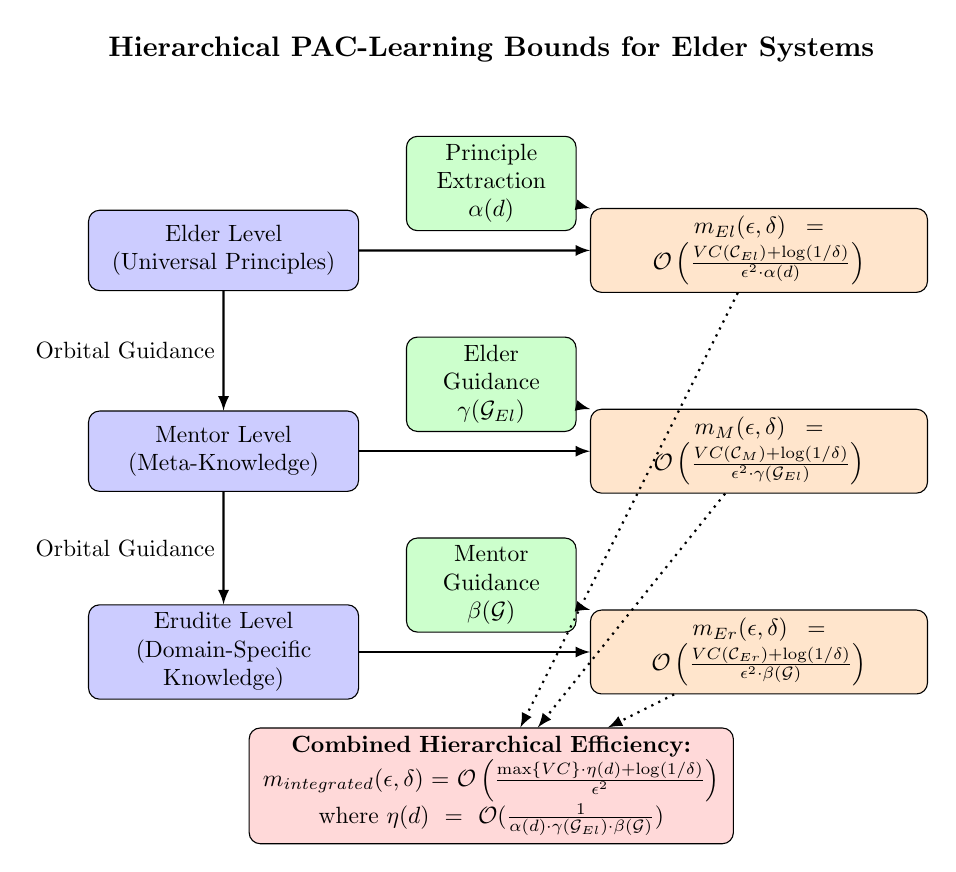
\begin{tikzpicture}[scale=0.85, transform shape]
    % Define styles
    \tikzset{
        level/.style={
            draw,
            fill=blue!20,
            rounded corners,
            minimum width=4cm,
            minimum height=1.2cm,
            text width=3.8cm,
            align=center
        },
        complexity/.style={
            draw,
            fill=orange!20,
            rounded corners,
            minimum width=5cm,
            minimum height=1.2cm,
            text width=4.8cm,
            align=center
        },
        arrow/.style={
            ->,
            thick,
            >=latex
        },
        factor/.style={
            draw,
            fill=green!20,
            rounded corners,
            minimum width=2.5cm,
            minimum height=1cm,
            text width=2.3cm,
            align=center
        }
    }
    
    % Hierarchy levels
    \node[level] (elder) at (0,6) {Elder Level\\(Universal Principles)};
    \node[level] (mentor) at (0,3) {Mentor Level\\(Meta-Knowledge)};
    \node[level] (erudite) at (0,0) {Erudite Level\\(Domain-Specific Knowledge)};
    
    % Sample complexity boxes
    \node[complexity] (elder_complex) at (8,6) {$m_{El}(\epsilon, \delta) = \mathcal{O}\left(\frac{\text{VC}(\mathcal{C}_{El}) + \log(1/\delta)}{\epsilon^2 \cdot \alpha(d)}\right)$};
    \node[complexity] (mentor_complex) at (8,3) {$m_{M}(\epsilon, \delta) = \mathcal{O}\left(\frac{\text{VC}(\mathcal{C}_{M}) + \log(1/\delta)}{\epsilon^2 \cdot \gamma(\mathcal{G}_{El})}\right)$};
    \node[complexity] (erudite_complex) at (8,0) {$m_{Er}(\epsilon, \delta) = \mathcal{O}\left(\frac{\text{VC}(\mathcal{C}_{Er}) + \log(1/\delta)}{\epsilon^2 \cdot \beta(\mathcal{G})}\right)$};
    
    % Efficiency factors
    \node[factor] (alpha) at (4,7) {Principle Extraction\\$\alpha(d)$};
    \node[factor] (gamma) at (4,4) {Elder Guidance\\$\gamma(\mathcal{G}_{El})$};
    \node[factor] (beta) at (4,1) {Mentor Guidance\\$\beta(\mathcal{G})$};
    
    % Vertical connections
    \draw[arrow] (elder) -- node[left] {Orbital Guidance} (mentor);
    \draw[arrow] (mentor) -- node[left] {Orbital Guidance} (erudite);
    
    % Horizontal connections
    \draw[arrow] (elder) -- (elder_complex);
    \draw[arrow] (mentor) -- (mentor_complex);
    \draw[arrow] (erudite) -- (erudite_complex);
    
    % Factor connections
    \draw[arrow, dashed] (alpha) -- (elder_complex);
    \draw[arrow, dashed] (gamma) -- (mentor_complex);
    \draw[arrow, dashed] (beta) -- (erudite_complex);
    
    % Combined efficiency
    \node[draw, fill=red!15, rounded corners, text width=7cm, align=center] (combined) at (4,-2) {
        \textbf{Combined Hierarchical Efficiency:}\\
        $m_{integrated}(\epsilon, \delta) = \mathcal{O}\left(\frac{\max\{\text{VC}\} \cdot \eta(d) + \log(1/\delta)}{\epsilon^2}\right)$\\
        where $\eta(d) = \mathcal{O}(\frac{1}{\alpha(d) \cdot \gamma(\mathcal{G}_{El}) \cdot \beta(\mathcal{G})})$
    };
    
    % Combined connections
    \draw[arrow, dotted, thick] (elder_complex) -- (combined);
    \draw[arrow, dotted, thick] (mentor_complex) -- (combined);
    \draw[arrow, dotted, thick] (erudite_complex) -- (combined);
    
    % Title
    \node[align=center, font=\bfseries, scale=1.2] at (4,9) {Hierarchical PAC-Learning Bounds for Elder Systems};
    
\end{tikzpicture}
\caption{Hierarchical PAC-Learning framework for the Elder system. Each level (Elder, Mentor, Erudite) has its own sample complexity bound, modified by efficiency factors ($\alpha$, $\gamma$, $\beta$) that capture the benefits of principle extraction, Elder guidance, and Mentor guidance respectively. The combined hierarchical efficiency $\eta(d)$ represents the compounded benefit of the entire system architecture, providing theoretical guarantees for sample efficiency that improve as the number of domains $d$ increases.}
\label{fig:hierarchical_pac}
\end{figure}